\section{Discussion}
We claim that our implementation is correct-by-construction because it is obviously correct because the code \textit{is} the model specification - we have closed the gap between the specification and its implementation. Still we need to verify the dynamics and test the system for its numerical behaviour under varying $\Delta t$.

\begin{figure}
	\centering
	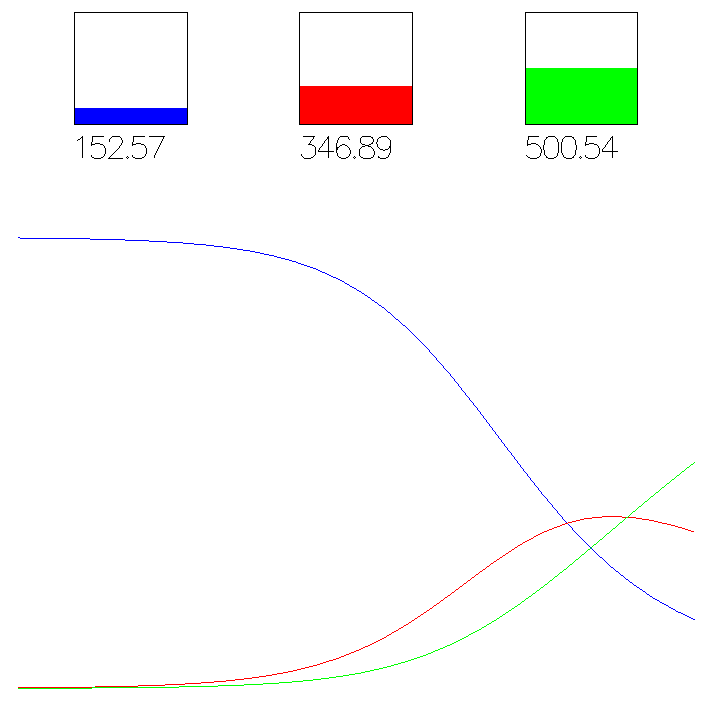
\includegraphics[width=.4\textwidth, angle=0]{./fig/visualisation_t50.png}
	\caption{Snapshot of a real-time visualisation of a SIR compartment model simulating using Haskell. Population Size $N$ = 1,000, contact rate $\beta =  \frac{1}{5}$, infection probability $\gamma = 0.05$, illness duration $\delta = 15$ with initially 1 infected agent. Simulation run until $t = 50$.}
	\label{fig:sir_sd_visualisation}
\end{figure}

TODO: argue why it is correct-by-construction, why reproducible guaranteed at compile-time,... support our initial hypothesis and claims from introduction

TODO: integral is the fundamental function
- need to show that it indeed implements the rectangle rule. 
- show that with too large dt we arrive at slightly different results after same time-steps
- implement a better integral function using better behaved numerical integration

\begin{center}
  \begin{tabular}{ c || c | c | c  }
    $\Delta t$ & Susceptibles & Infected & Recovered \\ \hline \hline 
    1.0 & 17.52 & 26.87 & 955.61 & 419.07 at t = 51 \\ \hline
    0.5 & 23.24 & 25.63 & 951.12 & 399.53 at t = 47.5 \\ \hline
    0.1 & 27.56 & 24.27 & 948.17 & 384.71 at t = 44.7 \\ \hline
    $1e-2$ & 28.52 & 24.11 & 947.36 & 381.48 at t = 43.97 \\ \hline
    $1e-3$ & 28.62 & 24.08 & 947.30 & 381.16 at t = 43.9 
    
    \label{tab:delta_influence}
  \end{tabular}
\end{center}

TODO: compare with an AnyLogic solution
- show picture and compare it with the initial one
- compare to anylogic run after t = 100 sus = 28.625, inf = 24.081, rec = 947.294, max inf = 381.132 at t = 44)